\documentclass[a4paper]{scrartcl}

\usepackage[usenames,dvipsnames]{xcolor}
\usepackage{amsmath,amssymb,amsfonts}
\usepackage{graphicx}

\title{Track an Object in 3D Space ReadMe}
\author{Philipp Rapp}
\date{\today}

\begin{document}

\maketitle

\section*{FP.0 Final Report}
\textcolor{gray}{\textit{Provide a Writeup / README that includes all the rubric points and how you addressed each one. You can submit your writeup as markdown or pdf.}}

The document at hand represents the readme file.

\section*{FP.1 Match 3D Objects}
\textcolor{gray}{\textit{Implement the method "matchBoundingBoxes", which takes as input both the previous and the current data frames and provides as output the ids of the matched regions of interest (i.e. the boxID property). Matches must be the ones with the highest number of keypoint correspondences.}}

As a first step, I changed the references to be \texttt{const} whenever possible.
That is nothing functional, but makes the code a bit safer.

In order to address the matching of the box identifiers, I decided to implement a greedy algorithm.
As a foundation, I set up a matrix which contains a row for every box ID in the previous frame,
and a column for every box ID in the current frame.
Every element of this matrix corresponds therefore represents a concatenation between two box identifiers
and therefore objects (vehicles).
The keypoint matches are now filled into this matrix.
Once the matrix is complete, I greedily select the elements with the largest number of keypoint matches.
The position in the matrix (row and column) then connects the box identifiers between the previous
and the current frame. Once a connection is established, the entire row and column is set to zero,
as this identifier pair has now been dealt with.

In order to get a better feeling for what is going on, I created some visual debug output in the
form of images, see Figure~\ref{fig:matching_3d_objects}.

\begin{figure}
	\centering
	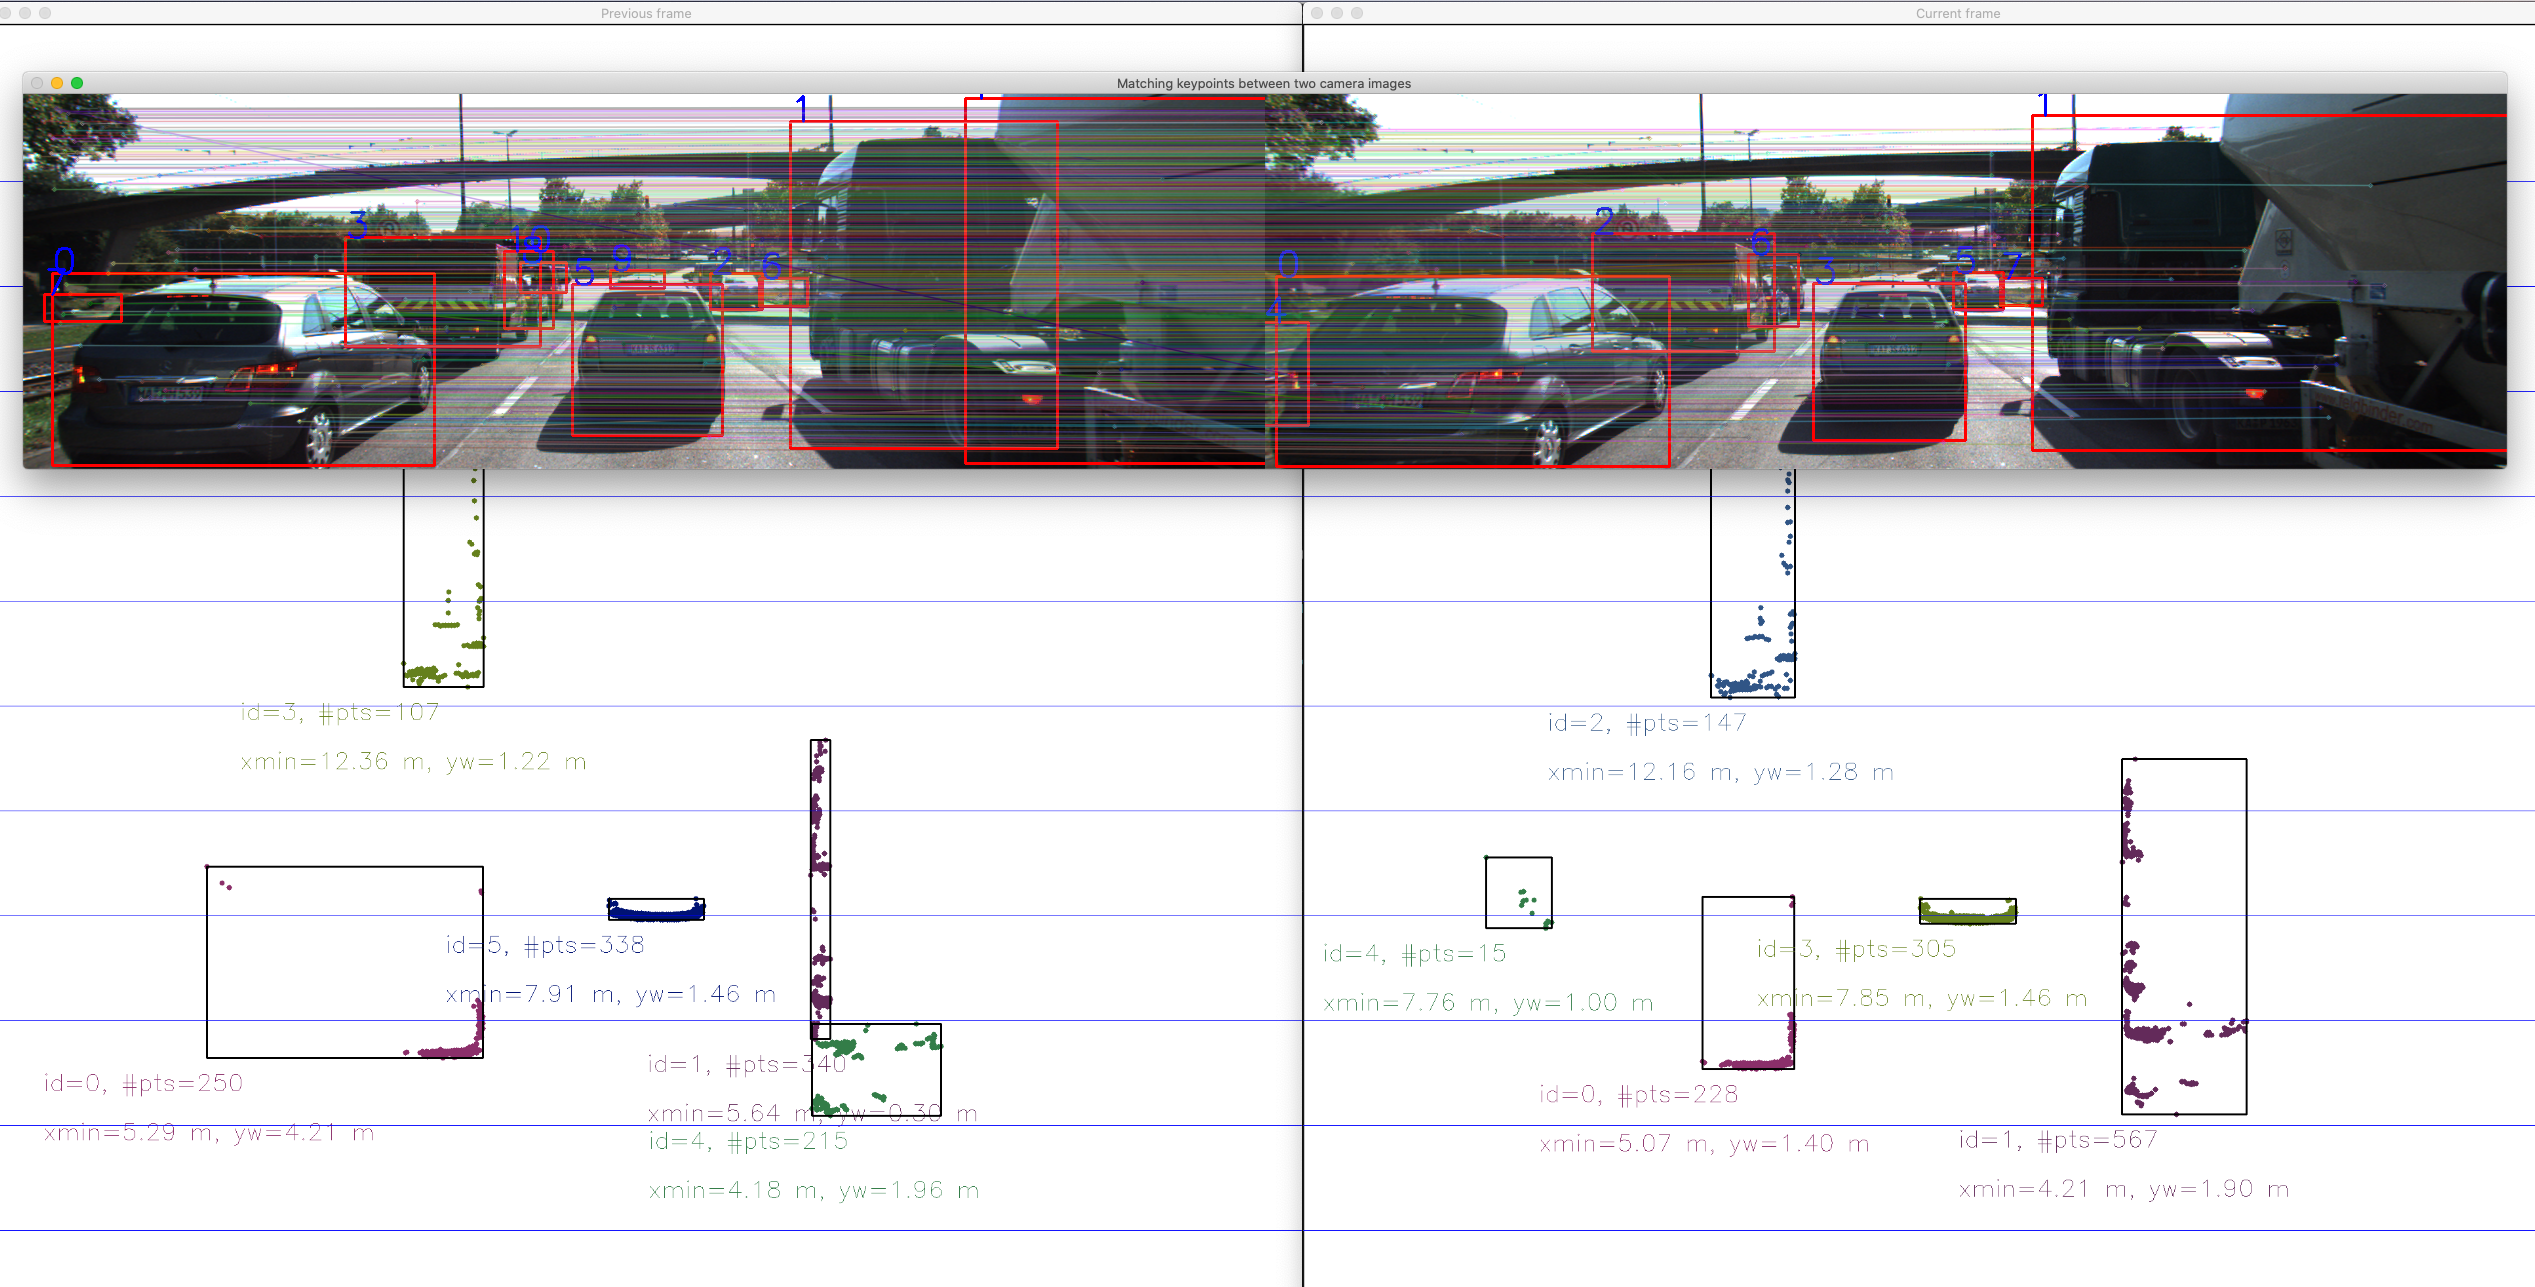
\includegraphics[width=0.8\columnwidth]{./img/3D_object_matching}
	\caption{Simultaneous visualization of the 3D top view from the previous and current frame,
		along with the keypoint descriptor matching, the latter being augmented by the
		2D bounding boxes.
		In this specific scene, the identifier of the leading vehicle changes
		from 5 to 3.}
	\label{fig:matching_3d_objects}
\end{figure}

\section*{FP.2 Compute Lidar-based TTC}
\textcolor{gray}{\textit{Compute the time-to-collision in second for all matched 3D objects using only Lidar measurements from the matched bounding boxes between current and previous frame. }}

According to lesson 2, the time-to-collision (TTC) based on a constant velocity model is
\begin{equation}
	t_\text{ttc} = \frac{d_1}{v_0} = \frac{d_1 \Delta t}{d_1 - d_0}
\end{equation}
with $d_0$ being the distance from our vehicle to the lead vehicle in the previous frame (index 0),
and $d_1$ being the distance from our vehicle to the lead vehicle in the current frame (index 1).
$v_0$ is the velocity. As it is a constant velocity model, $v_0 = v_1$.
$\Delta t$ is the step size, i.e., the difference between the time stamps of
the individual measurements. $\Delta t$ is the reciprocal of the frame rate.

The current model for the vehicle extent consists of axis-aligned bounding boxes.
In other words, any (non-zero) orientation of the vehicles as well as
curvature on their boundary is neglected.
For this reason, it is valid to assume that the tail of the vehicles can be represented
by a plane with a normal vector which is pointing along the ego vehicle's $x$-axis
($x$ pointing forward in accordance with ISO 8855 and as used throughout this course).
This in turn allows us to use the plane fitting RANSAC from the Lidar course
in order to robustly estimate the tail of the lead vehicle, thereby removing outliers, as
can be seen in Figure~\ref{fig:lidar_ransac}.
I included my Lidar code into the project, slightly adapted for the Camera course data types, in order
to compute the RANSAC. The point cloud library is not needed.

\begin{figure}
	\centering
	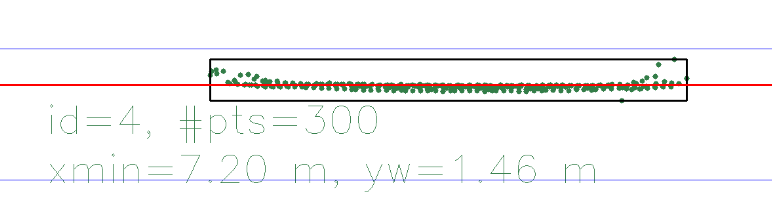
\includegraphics[width=0.8\columnwidth]{./img/lidar_ransac_vehicle_tail}
	\caption{Estimation of the tail of the lead vehicle by means of plane
			fitting using RANSAC. The plane is constrained to have
			a normal vector which is pointing along the $x$-axis.
			In the top view, the red line represents the plane.
			Note how the outlier in the bottom right region enlarges
			the bounding box, but is rejected by the plane fit.}
	\label{fig:lidar_ransac}
\end{figure}


\section*{FP.3 Associate Keypoint Correspondences with Bounding Boxes}
\textcolor{gray}{\textit{Prepare the TTC computation based on camera measurements by associating keypoint correspondences to the bounding boxes which enclose them. All matches which satisfy this condition must be added to a vector in the respective bounding box.}}

\section*{FP.4 Compute Camera-based TTC}
\textcolor{gray}{\textit{Compute the time-to-collision in second for all matched 3D objects using only keypoint correspondences from the matched bounding boxes between current and previous frame.}}

\section*{FP.5 Performance Evaluation 1}
\textcolor{gray}{\textit{Find examples where the TTC estimate of the Lidar sensor does not seem plausible. Describe your observations and provide a sound argumentation why you think this happened.}}

\section*{FP.6 Performance Evaluation 2}
\textcolor{gray}{\textit{Run several detector / descriptor combinations and look at the differences in TTC estimation. Find out which methods perform best and also include several examples where camera-based TTC estimation is way off. As with Lidar, describe your observations again and also look into potential reasons.}}


\end{document}